\chapter{Improving SUDS}

\section{Implementing digital signatures -- SudsSigner}

\subsection{Internal structure}

The internal structure of the plugin can be seen on Figure \ref{fig:cdSudsSigner}, the stereotypes describe the functionality (component or binding) and the runtime environment (Python or native) of each component. Native components are preferred for their reusability and performance -- reusable components are tested more thoroughly, as more projects can depend on them, which makes them less prone to errors, thus more suitable for security-critical tasks, such as cryptography (OpenSSL). From a performance point of view, XML parsing and processing is also a task, that is better done using native and mature code (libxml2) because of its complexity. Python, on the other hand, is more suitable for the purpose of connecting components together, and describe high-level business logic in a readable and portable way.

\begin{figure}[htbp]
 \centering
 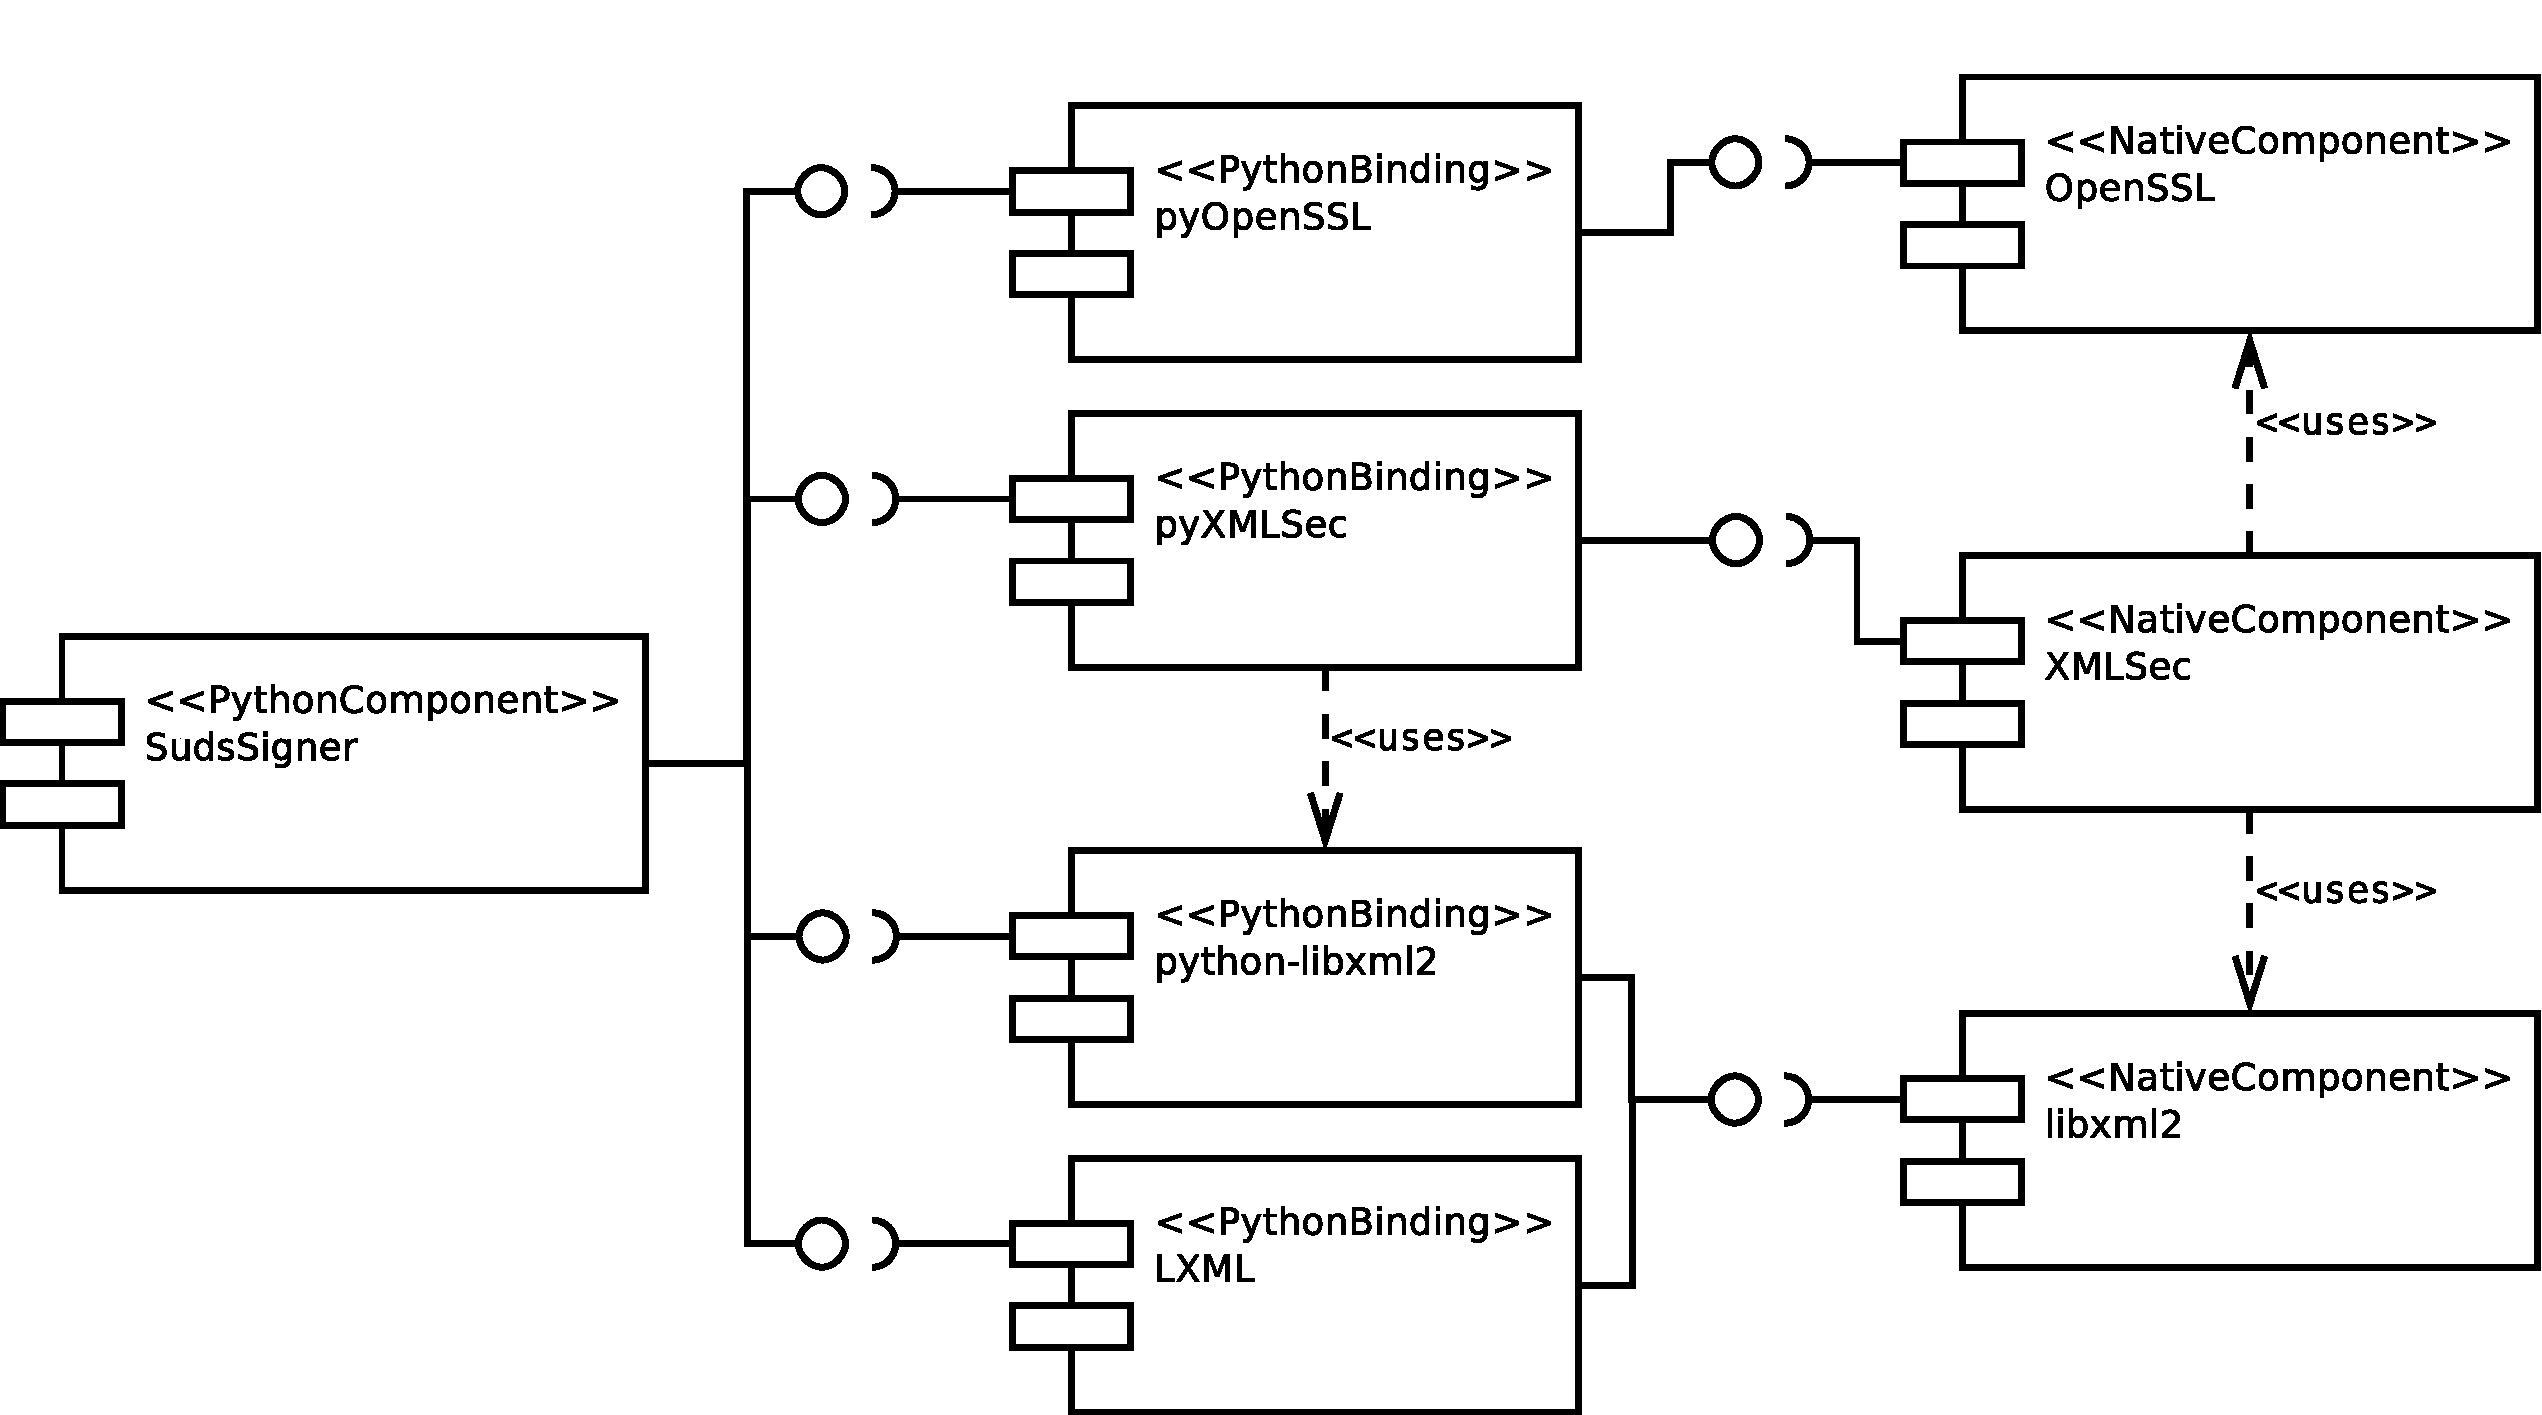
\includegraphics[width=\textwidth]{images/cdSudsSigner.pdf}
 \caption{Component diagram of the SudsSigner plugin}
 \label{fig:cdSudsSigner}
\end{figure}

\subsection{Components used}

\subsubsection{Libxml2, python-libxml2 and LXML}

``Libxml2 is the XML C parser and toolkit developed for the Gnome project (but usable outside of the Gnome platform), it is free software available under the MIT License.''\cite{libxml2-homepage} This sentence summarizes the project pretty well -- it's written in C, which is a good compromise between performance, portability and usability, and it's available under the MIT license, which makes it possible to either bundle it to FLOSS projects or redistribute it with proprietary software. Since many projects depend on it, the quality of the code is high, and it passes all of the OASIS XML Tests Suite.

Python-libxml2 provides low-level Python bindings to access all of the functionality of libxml2. It has the advantages that the developer gets the full power of libxml2, but the interface resembles the original C API, which causes longer development and debug cycles. On the other hand, LXML wraps libxml2 in modules and classes providing a powerful high-level interface, which is more suitable for quick prototyping and maintainable codebase.

I chose this combination because no other combination can offer the perfomance of the native parsing and processing engine combined with so rich and powerful Python interface.

\subsubsection{OpenSSL and pyOpenSSL}

``The OpenSSL Project is a collaborative effort to develop a robust, commercial-grade, full-featured, and Open Source toolkit implementing [\ldots] a full-strength general purpose cryptography library''\cite{openssl-homepage} This library is also written in C, has a unique Apache and BSD-like license, and is FIPS 140-2 compliant. PyOpenSSL provides a friendly object-oriented interface, which makes it possible to access all the functionality of OpenSSL I needed. It's also well-maintained, which makes installing it on modern OSes a breeze. I chose this duo, because it seemed the only solution capable of handling PEM files in all the ways I needed.

\subsubsection{XMLSec and PyXMLSec}

XMLSec is a C library based on Libxml2 and supports XML signature, encryption, and canonicalization.\cite{xmlsec-homepage} It's released under the MIT license, and is still maintained, so most Linux distributions provide it as an easily installable package. It uses libxml2 for XML processing and it can use several cryptography backends (OpenSSL, GnuTLS, Libgcrypt, NSS) for signature creation and encryption.

Python bindings were created for the Glasnost project financed by the French Department of Economy, Finance and Industry in 2003, but development seems to ceased around 2005. The bindings are still working, only one feature needed a patch sent to the mailing list of the project in 2010. The documentation consists of a dozen examples and an API reference generated from the source code, so the use of these bindings require quite a bit of experimentation.

There are few other projects trying to create XML signatures, with not much success, so I chose this one, because at least it worked, and with a bit of work, I managed to make it do what I wanted.
